%%%%%%%%%%%%%%%%%%%%%%%%%%%%%%%%
% Chapter 3. Experimental Analysis
%%%%%%%%%%%%%%%%%%%%%%%%%%%%%%%%

\section{Experimental Analysis}\label{sec:experimental_analysis}

% ================================================================
\subsection{Random Soft Prompt: Definition and Setup}\label{sec:rsp_definition}
% ================================================================

Let $\mathbf{W}_E \in \mathbb{R}^{V \times d}$ denote the token embedding matrix of a pretrained LLM, where $V$ is the vocabulary size and $d$ is the hidden dimension. We define an RSP $\mathbf{H} = [h_1, \dots, h_L] \in \mathbb{R}^{L \times d}$ as a sequence of $L$ continuous vectors, where each vector is independently sampled from:
\begin{equation}
  h_j \sim \mathcal{N}(\mu_E,\; \sigma_E^2 \mathbf{I}), \quad j = 1, \dots, L,
\end{equation}
with $\mu_E = \frac{1}{Vd}\sum_{i,k} [\mathbf{W}_E]_{i,k}$ and $\sigma_E = \mathrm{std}(\mathbf{W}_E)$. Let $\mathbf{X} = [x_1, \dots, x_T] \in \mathbb{R}^{T \times d}$ denote the embedding sequence of the original input. The RSP-augmented input $\tilde{\mathbf{X}}$ is constructed by concatenating $\mathbf{H}$ with $\mathbf{X}$ at one of three positions without modifying the original prompt text: \textit{prefix} ($[\mathbf{H}; \mathbf{X}]$), \textit{infix} ($\mathbf{H}$ inserted within $\mathbf{X}$), or \textit{suffix} ($[\mathbf{X}; \mathbf{H}]$), following the injection strategies adopted in prior work \citep{kang2025model, xu2025softcot, ye2025thinking, zhang2025memgen}. Sampling a new $\mathbf{H}$ for each batch ensures that the results are not dependent on any realization of the random embeddings.

We evaluate on three mathematical reasoning benchmarks: MATH-500 \citep{lightman2024lets}, GSM8K \citep{cobbe2021training}, and AIME24, using LLaMA-3.1-8B-Instruct \citep{grattafiori2024llama} and the Qwen2.5-Math model family \citep{yang2024qwen25math} across seven configurations including instruct models, base models, and base models with mismatched chat templates. All experiments use greedy decoding to isolate the effect of RSPs from sampling stochasticity. Only the final answer is evaluated through a fallback-based extraction pipeline. Full experimental details are provided in Appendix~\ref{app:setup}.

% ================================================================
\subsection{Does RSP Degrade Reasoning Performance?}\label{sec:performance}
% ================================================================

\begin{table}[!t]
\centering
\caption{Accuracy (\%) across model configurations and benchmarks. RSP reports the best result across injection positions (Prefix, Infix, Suffix); full per-position breakdown is in Appendix~\ref{app:ablation}. Values in parentheses indicate the difference from the baseline.}
\label{tab:performance}
\footnotesize
\setlength{\tabcolsep}{4pt}
\renewcommand{\arraystretch}{0.9}
\begin{tabular}{l cc cc cc}
\toprule
 & \multicolumn{2}{c}{\textbf{MATH-500}} & \multicolumn{2}{c}{\textbf{GSM8K}} & \multicolumn{2}{c}{\textbf{AIME24}} \\
\cmidrule(lr){2-3} \cmidrule(lr){4-5} \cmidrule(lr){6-7}
\textbf{Model} & Baseline & \cellcolor{blue!10}RSP & Baseline & \cellcolor{blue!10}RSP & Baseline & \cellcolor{blue!10}RSP \\
\midrule
\multicolumn{7}{l}{\textit{Instruct Models}} \\
\midrule
LLaMA-3.1-8B-Inst      & 52.20 & \cellcolor{blue!10}49.40 {\scriptsize($-$2.8)}  & 85.75 & \cellcolor{blue!10}86.73 {\scriptsize(+1.0)}  & 6.67  & \cellcolor{blue!10}10.00 {\scriptsize(+3.3)}  \\
Qwen2.5-Math-7B-Inst   & 83.20 & \cellcolor{blue!10}84.20 {\scriptsize(+1.0)}   & 95.45 & \cellcolor{blue!10}95.68 {\scriptsize(+0.2)}  & 13.33 & \cellcolor{blue!10}16.67 {\scriptsize(+3.3)}  \\
Qwen2.5-Math-1.5B-Inst & 73.00 & \cellcolor{blue!10}75.20 {\scriptsize(+2.2)}   & 85.29 & \cellcolor{blue!10}85.75 {\scriptsize(+0.5)}  & 10.00 & \cellcolor{blue!10}20.00 {\scriptsize(+10.0)} \\
\midrule
\multicolumn{7}{l}{\textit{Base Models (Raw Text)}} \\
\midrule
Qwen2.5-Math-7B        & 72.20 & \cellcolor{blue!10}71.60 {\scriptsize($-$0.6)}  & 84.15 & \cellcolor{blue!10}84.31 {\scriptsize(+0.2)}  & 6.67  & \cellcolor{blue!10}16.67 {\scriptsize(+10.0)} \\
Qwen2.5-Math-1.5B      & 61.40 & \cellcolor{blue!10}64.40 {\scriptsize(+3.0)}   & 77.86 & \cellcolor{blue!10}74.30 {\scriptsize($-$3.6)} & 16.67 & \cellcolor{blue!10}10.00 {\scriptsize($-$6.7)} \\
\midrule
\multicolumn{7}{l}{\textit{Base Models + ChatML (Format Mismatch)}} \\
\midrule
Qwen2.5-Math-7B        & 52.20 & \cellcolor{blue!10}70.40 {\scriptsize(+18.2)}  & 58.30 & \cellcolor{blue!10}75.97 {\scriptsize(+17.7)} & 23.33 & \cellcolor{blue!10}23.33 {\scriptsize(+0.0)}  \\
Qwen2.5-Math-1.5B      & 34.40 & \cellcolor{blue!10}63.40 {\scriptsize(+29.0)}  & 37.45 & \cellcolor{blue!10}67.02 {\scriptsize(+29.6)} & 13.33 & \cellcolor{blue!10}20.00 {\scriptsize(+6.7)}  \\
\bottomrule
\end{tabular}
\end{table}

We first examine how injecting random embeddings affects the model's reasoning performance. Table~\ref{tab:performance} reports the accuracy for each model configuration, using the best RSP result across injection positions (Prefix, Infix, Suffix) and $L \in \{10, 15, 20\}$ for each benchmark.

For instruct models and base models with their native prompt formats, RSP injection maintains or slightly shifts baseline performance within a few percentage points. Most strikingly, under prompt-format mismatch --- where base models receive ChatML templates they were not trained on --- RSP yields pronounced improvements of up to $+29$\%p. These gains are difficult to attribute to simple perturbation effects, as noise that merely raises model uncertainty would further degrade performance.

\begin{table}[!t]
\centering
\caption{Comparison with existing soft prompt methods (TTSV, SoftCoT, LTPO) under unified evaluation. Baseline and RSP values are from Table~\ref{tab:performance}. \textbf{Bold} denotes the best result and \underline{underline} denotes the second best for each model--benchmark pair.}
\label{tab:prior_comparison}
\footnotesize
\renewcommand{\arraystretch}{0.9}
\begin{tabular}{llccccc}
\toprule
\textbf{Model} & \textbf{Benchmark} & \textbf{Baseline} & \cellcolor{blue!10}\textbf{RSP} & \textbf{TTSV} & \textbf{SoftCoT} & \textbf{LTPO} \\
\midrule
\multirow{3}{*}{Qwen2.5-Math-7B-Instruct} & MATH-500 & 83.20 & \cellcolor{blue!10}\textbf{84.20} & \underline{83.80} & 82.80 & 83.00 \\
 & GSM8K   & \underline{95.45} & \cellcolor{blue!10}\textbf{95.68} & 95.30 & 95.00 & 94.84 \\
 & AIME24  & 13.33 & \cellcolor{blue!10}\underline{16.67} & \textbf{23.30} & \underline{16.67} & 13.33 \\
\midrule
\multirow{3}{*}{Qwen2.5-Math-1.5B-Instruct} & MATH-500 & 73.00 & \cellcolor{blue!10}\underline{75.20} & \underline{75.20} & \textbf{76.00} & 72.40 \\
 & GSM8K   & 85.29 & \cellcolor{blue!10}\textbf{85.75} & \underline{85.70} & 84.46 & 84.53 \\
 & AIME24  & \underline{10.00} & \cellcolor{blue!10}\textbf{20.00} &  6.70 &  6.67 & \underline{10.00} \\
\bottomrule
\end{tabular}
\end{table}

We compare RSPs with prior soft prompt methods (TTSV, SoftCoT, LTPO) that optimize their embeddings for distinct objectives, under a unified evaluation protocol reported in Table~\ref{tab:prior_comparison}. All methods are re-evaluated with a shared answer extraction pipeline that applies fallback strategies, enabling a format-agnostic comparison despite each method's distinct prompt format and grading scheme. The results place RSPs on par with the optimized methods without requiring any training.

% ================================================================
\subsection{How Does RSP Affect the Output Distribution?}\label{sec:entropy}
% ================================================================

We analyze how RSP injection changes the model's output distribution during generation on Qwen2.5-Math-1.5B-Instruct with MATH-500, measuring per-token entropy, top-1 probability, and varentropy across the generation process. Figure~\ref{fig:entropy_first5} and Table~\ref{tab:entropy_first5} compare these metrics for the first 5\% of generation steps across RSP variants and prior soft prompt methods.

\begin{figure}[ht]
  \centering
  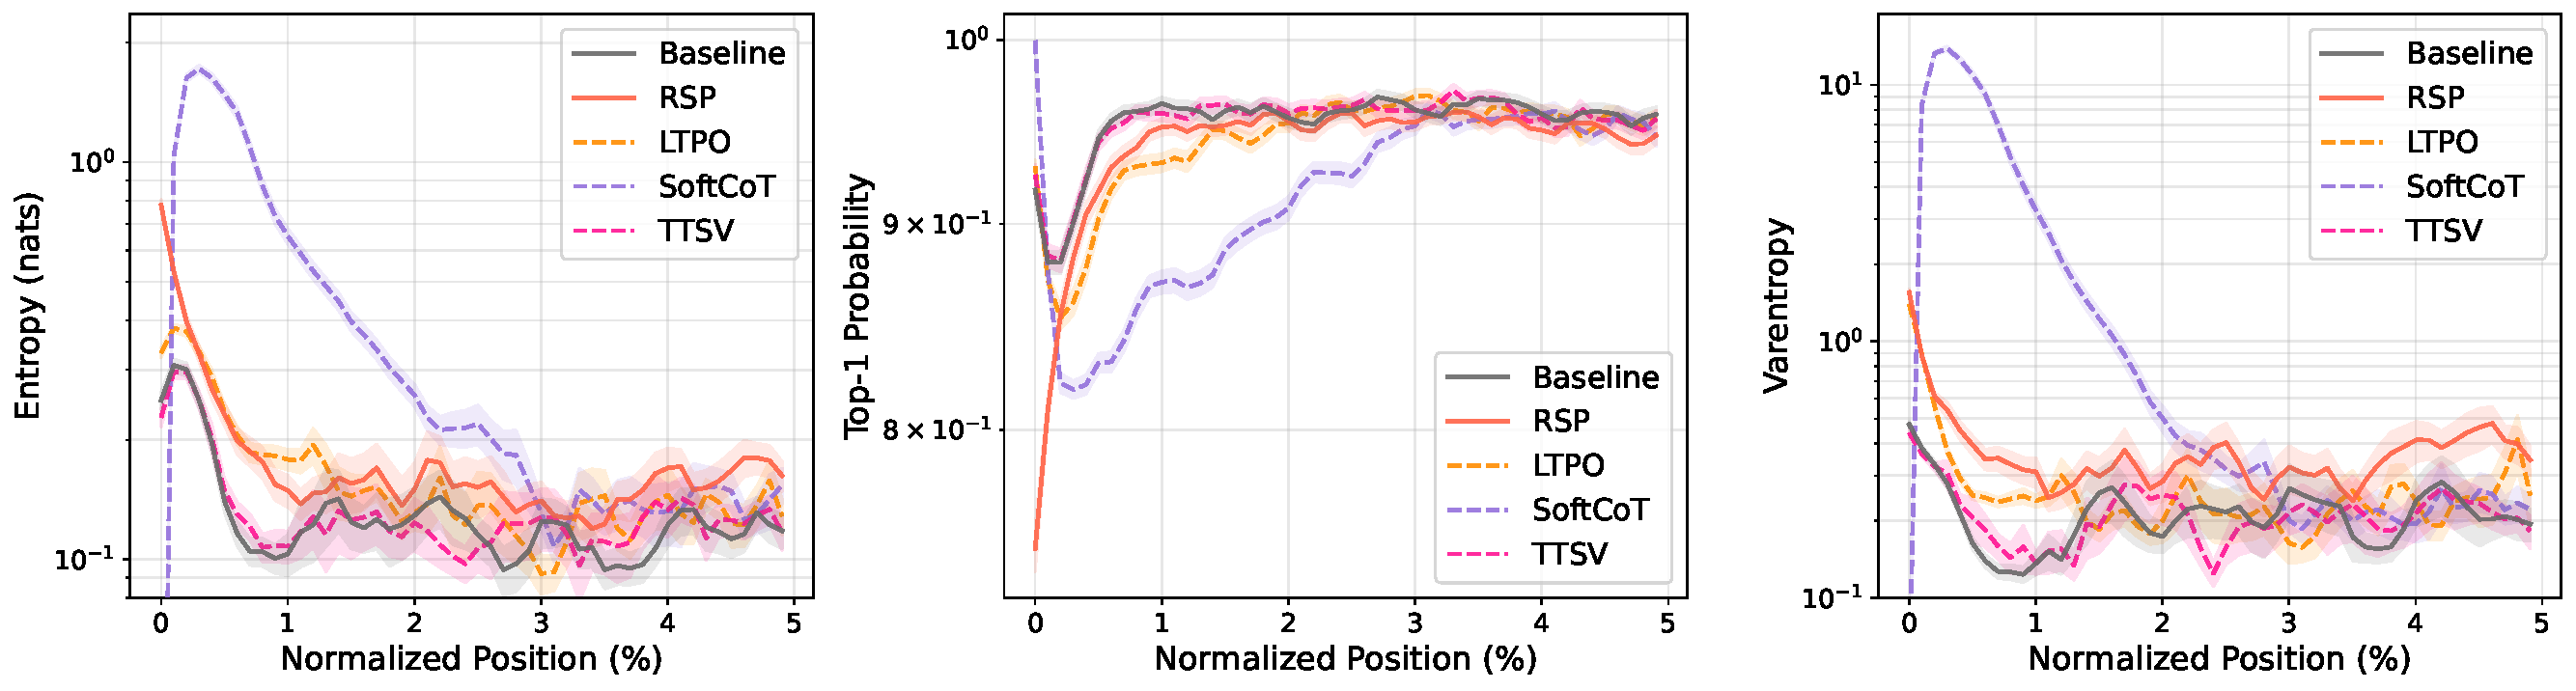
\includegraphics[width=\textwidth]{img/entropy/entropy_first5pct_zoom.pdf}
  \caption{Mean entropy, top-1 probability, and varentropy during the first 5\% of generation steps (Qwen2.5-Math-1.5B-Instruct, MATH-500). Shading indicates $\pm$1 SEM. Solid lines: RSP variants and the baseline. Dashed lines: existing soft prompt methods (LTPO, SoftCoT, TTSV).}
  \label{fig:entropy_first5}
\end{figure}

\begin{table}[ht]
\centering
\caption{Mean entropy, top-1 probability, and varentropy for the first 5\% of generation steps (Qwen2.5-Math-1.5B-Instruct, MATH-500).}
\label{tab:entropy_first5}
\small
\begin{tabular}{lccccccc}
\toprule
\textbf{Metric} & \textbf{Baseline} & \cellcolor{blue!10}\textbf{Prefix} & \cellcolor{blue!10}\textbf{Infix} & \cellcolor{blue!10}\textbf{Suffix} & \textbf{LTPO} & \textbf{SoftCoT} & \textbf{TTSV} \\
\midrule
Entropy & 0.1332 & \cellcolor{blue!10}0.1366 & \cellcolor{blue!10}0.1402 & \cellcolor{blue!10}0.1941 & 0.1662 & 0.4218 & 0.1359 \\
Top-1 Prob & 0.9535 & \cellcolor{blue!10}0.9523 & \cellcolor{blue!10}0.9525 & \cellcolor{blue!10}0.9373 & 0.9437 & 0.9156 & 0.9534 \\
Varentropy & 0.2181 & \cellcolor{blue!10}0.2207 & \cellcolor{blue!10}0.2463 & \cellcolor{blue!10}0.4010 & 0.2953 & 2.2234 & 0.2174 \\
\bottomrule
\end{tabular}
\end{table}

These results show that RSP modifies the early-stage output distribution across all injection positions: entropy increases (the token distribution flattens), top-1 probability decreases (commitment to a dominant token weakens), and varentropy increases (indicating multimodal distributions \citep{ahmed2026logitscope}). High-entropy positions are known to act as critical forking points that determine reasoning trajectories \citep{wang2025beyond}, so this shift moves the model toward a state where multiple reasoning paths can coexist. The change is localized to the initial reasoning stage; in the middle and final portions of generation, all three metrics converge to baseline levels.

Although existing soft prompt methods are optimized for different objectives, they share a common pattern of increasing early-stage entropy. Notably, TTSV, which optimizes soft prompts using a reward that reduces the mean entropy of reasoning trajectories, still exhibits early entropy comparable to the baseline. This suggests that elevating early-stage entropy is an inherent effect of injecting non-pretrained continuous embeddings, independent of the optimization objective.

% ================================================================
\subsection{Does RSP Induce Trajectory Diversity?}\label{sec:diversity}
% ================================================================

Section~\ref{sec:entropy} empirically established that RSP reshapes the early-stage output distribution. We now examine whether this shift translates into reasoning diversity at three complementary levels of analysis: token rankings, semantic content of trajectories, and task-level outcomes. All three analyses share the setting: Qwen2.5-Math-1.5B-Instruct, MATH-500, suffix injection, and $L=10$.

\paragraph{Token-level: distribution beyond temperature.}
\begin{wraptable}{r}{0.42\textwidth}
  \vspace{-1.2em}
  \centering
  \caption{First-token distribution metrics measured against the baseline at $\tau{=}1.0$, comparing the baseline at $\tau{=}2.0$ with RSP at $\tau{=}1.0$.}
  \label{tab:rsp_vs_temp}
  \footnotesize
  \setlength{\tabcolsep}{4pt}
  \renewcommand{\arraystretch}{0.9}
  \begin{tabular}{lcc}
    \toprule
    \textbf{Metric} & \textbf{$\tau{=}2.0$} & \cellcolor{blue!10}\textbf{RSP} \\
    \midrule
    Spearman $\rho$ & 1.0 & \cellcolor{blue!10}\textbf{0.651} \\
    Mass outside top-10 & 5.15\% & \cellcolor{blue!10}\textbf{27.64\%} \\
    JS divergence & 0.086 & \cellcolor{blue!10}\textbf{0.231} \\
    \bottomrule
  \end{tabular}
\end{wraptable}
Under autoregressive decoding, any trajectory-level divergence between RSP and the baseline must originate from the first generation step, a critical forking point for reasoning trajectories \citep{wang2025beyond}. Using the baseline at $\tau{=}1.0$ as reference, we compare RSP at $\tau{=}1.0$ against the baseline at $\tau{=}2.0$ (the high-temperature ceiling of what flattening alone can achieve) on three complementary metrics: Spearman rank correlation $\rho$ to detect rank reorganization, the probability mass placed outside the baseline's top-10 to measure support expansion, and Jensen--Shannon divergence to quantify the overall magnitude of distributional change (formal definitions in Appendix~\ref{app:token_metrics}).

Table~\ref{tab:rsp_vs_temp} reports the contrast. Even at $\tau{=}2.0$, only 5.15\% of probability mass falls outside the baseline's top-10; RSP at $\tau{=}1.0$ reaches 27.64\%. The Spearman rank correlation tells the story more starkly: because temperature scaling $p_i^{(\tau)} \propto p_i^{1/\tau}$ is a monotone transform that preserves token ranking ($p_i > p_j \iff p_i^{(\tau)} > p_j^{(\tau)}$) for any $\tau > 0$, $\rho$ relative to the baseline is exactly $1$ as a mathematical identity. RSP, by contrast, reranks the token distribution itself, reducing $\rho$ to $0.651$---an effect temperature cannot produce at any $\tau$. The Jensen--Shannon divergence ($0.231$) quantifies the overall magnitude of this distributional change. Since $\rho < 1$ rules out rank-preserving flattening as the sole cause, the high divergence reflects a structural reshape of the distribution rather than a uniform flattening of the same ranking.

% =====================================================================
% Reranking-by-position analysis (commented out for now; may be added back).
% Original Token-level paragraph + Table 4 (matched-context, 50-step decay).
% =====================================================================
%
% \paragraph{Token-level: reranking analysis.}
% We first ask whether RSP genuinely alters token rankings, beyond the distributional smoothing shown in Section~\ref{sec:entropy}. Under matched-context comparison on 500 MATH-500 problems with 32 RSP seeds, we compare RSP's greedy argmax against the baseline's top-100 logits at the same token position, isolating the effect of embedding injection from trajectory drift.
%
% \begin{table}[ht]
% \centering
% \caption{Reranking breakdown by token position (32 RSP seeds, greedy). Each row reports the percentage of RSP argmax tokens that differ from the baseline top-1, decomposed by where they appear in the baseline's ranking. \textbf{Total} = sum of the four destination columns.}
% \label{tab:reranking}
% \footnotesize
% \renewcommand{\arraystretch}{0.9}
% \begin{tabular}{lccccc}
% \toprule
% \textbf{Position} & \textbf{Total} & \textbf{$\to$ top-2} & \textbf{$\to$ top-3--5} & \textbf{$\to$ top-6--10} & \textbf{$\to$ outside top-10} \\
% \midrule
% First token ($t=1$) & 23.07\% & 1.29\% & 0.03\% & 0.03\% & \textbf{21.71\%} \\
% Second token ($t=2$) & 4.22\% & \textbf{3.69\%} & 0.53\% & 0.00\% & 0.00\% \\
% Third token ($t=3$) & 2.10\% & \textbf{1.98\%} & 0.13\% & 0.00\% & 0.00\% \\
% Remaining tokens ($t=4,\dots,50$) & 1.36\% & \textbf{1.26\%} & 0.09\% & 0.003\% & 0.003\% \\
% \bottomrule
% \end{tabular}
% \end{table}
%
% Table~\ref{tab:reranking} reveals that RSP's reranking is concentrated at the first token. At $t=1$, 23.07\% of RSP samples select a token different from the baseline top-1, and 94\% of these fall outside the baseline's top-10. Beyond the first token, the total reranking rate drops sharply and the remaining reranking is confined almost entirely to the top-2, indicating that RSP's influence on later tokens is limited to local neighbors rather than new subtrees.

\paragraph{Trajectory-level: semantic diversity.}
\begin{wraptable}{r}{0.34\textwidth}
  \vspace{-1.2em}
  \centering
  \caption{Semantic diversity metrics averaged across the 64 problems.}
  \label{tab:semantic_metrics}
  \footnotesize
  \setlength{\tabcolsep}{4pt}
  \renewcommand{\arraystretch}{0.9}
  \begin{tabular}{lcc}
    \toprule
    \textbf{Metric} & \textbf{Baseline} & \cellcolor{blue!10}\textbf{RSP} \\
    \midrule
    Pairwise cos.\ dist. & 0.0612 & \cellcolor{blue!10}\textbf{0.0879} \\
    Inter-cluster dist. & 0.0183 & \cellcolor{blue!10}\textbf{0.0982} \\
    Intra-cluster dist. & 0.0526 & \cellcolor{blue!10}0.0528 \\
    \bottomrule
  \end{tabular}
\end{wraptable}
Token-level reranking raises a second question: do first-token perturbations produce semantically distinct reasoning paths, or do independently perturbed trajectories converge to the same solution strategy? We randomly sample 64 problems from MATH-500 and generate 300 independent trajectories per problem under two conditions, Baseline and RSP, with temperature $\tau = 1.0$. The trajectories are embedded via BGE-M3 \citep{chen2024bge} and compared on three metrics: mean pairwise cosine distance within each problem, inter-cluster distance between DBSCAN \citep{ester1996density} centroids, and intra-cluster distance. Table~\ref{tab:semantic_metrics} shows that RSP substantially increases the inter-cluster distance while leaving the intra-cluster distance unchanged: clusters become more separated while reasoning within each cluster remains consistent. RSP also wins on pairwise distance in 56 of 64 problems (87.5\%).

\begin{figure}[ht]
  \centering
  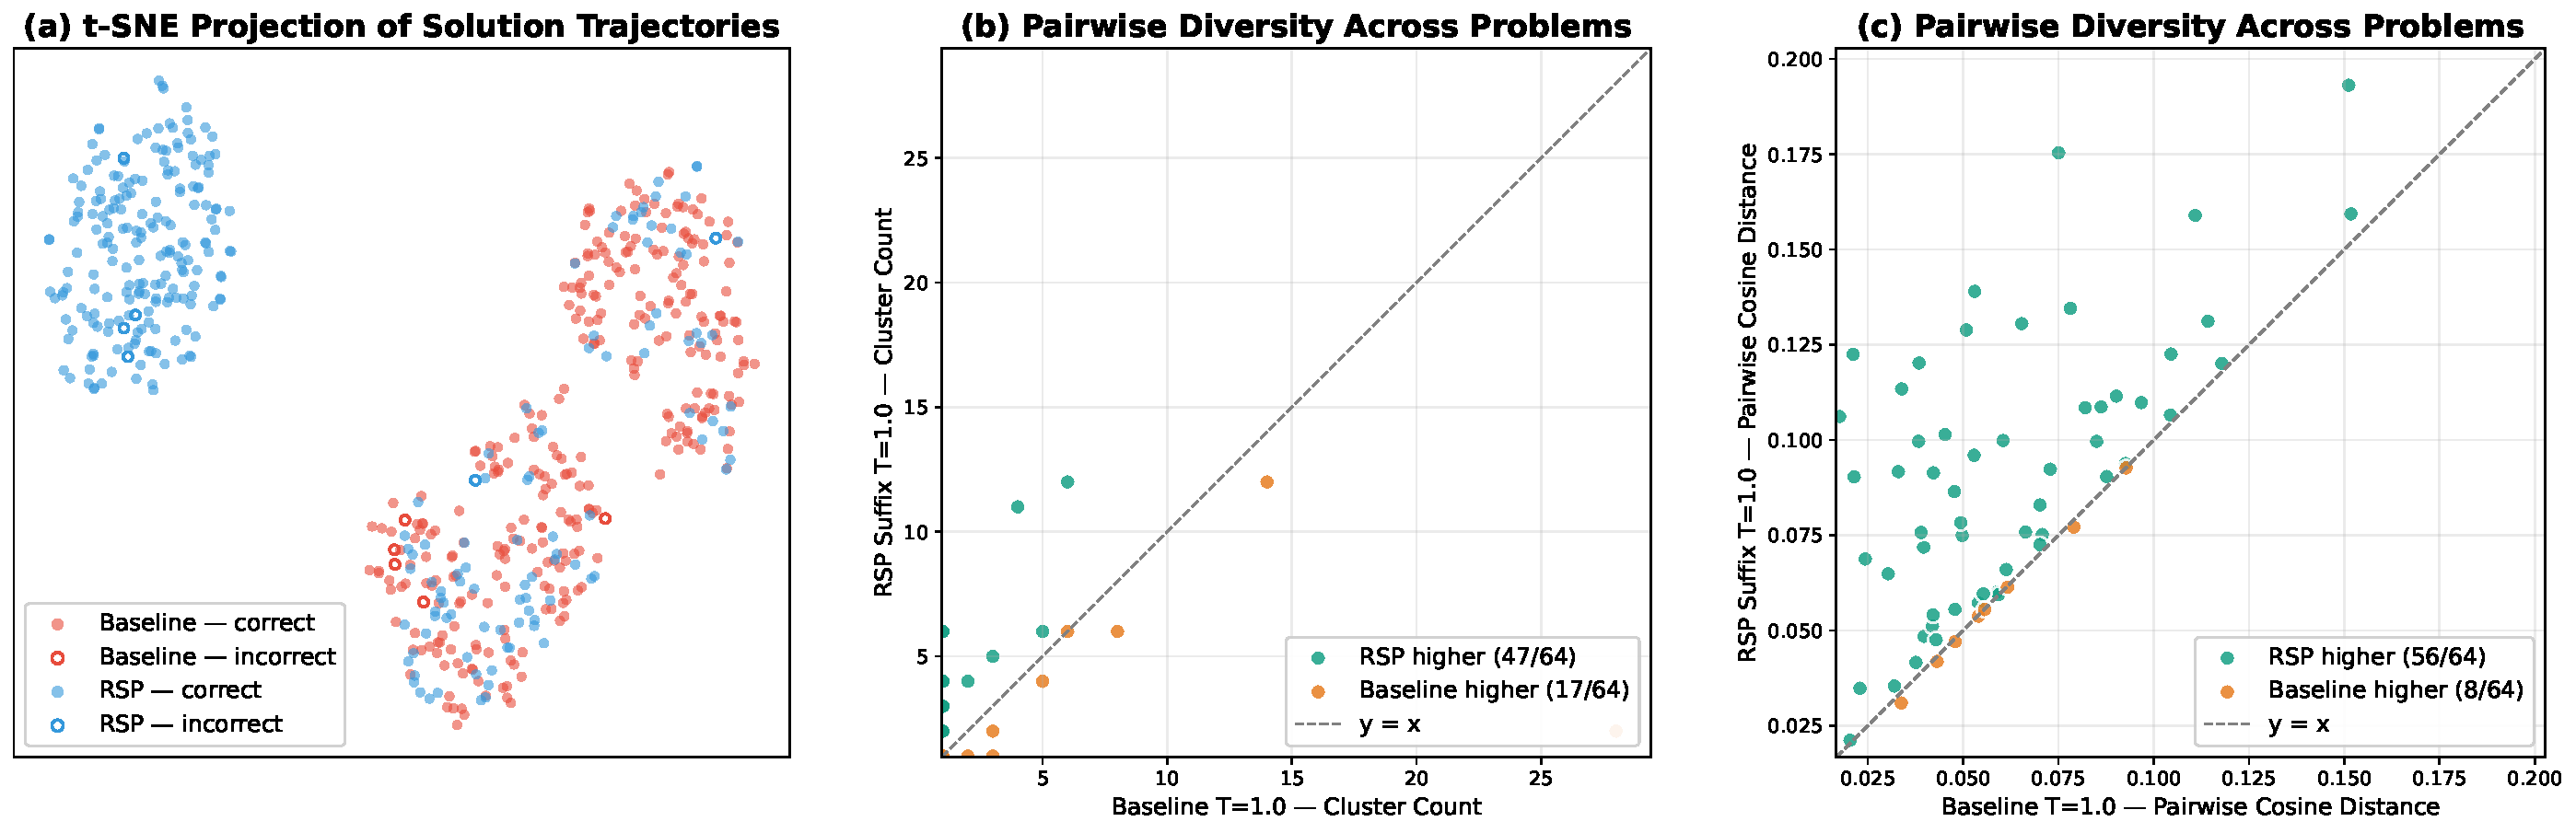
\includegraphics[width=\textwidth]{img/diversity/semantic_3panel.pdf}
  \caption{Semantic diversity analysis on 64 randomly sampled MATH-500 problems with 300 trajectories per condition (Qwen2.5-Math-1.5B-Instruct, $\tau=1.0$, BGE-M3 embeddings). (a) t-SNE projection for one representative problem (\texttt{test/prealgebra/951}): baseline (red) concentrates around one region while RSP suffix (blue) spreads across distinct clusters; filled markers denote correct answers and open markers denote incorrect. (b) Per-problem mean pairwise cosine distance; points above the diagonal indicate RSP produces more diverse trajectories than baseline. (c) Per-problem DBSCAN cluster count; RSP yields more distinct clusters than baseline on most problems.}
  \label{fig:semantic_diversity}
\end{figure}

Figure~\ref{fig:semantic_diversity}(a) illustrates the qualitative difference for the representative problem: the RSP samples (blue) cover the region occupied by baseline samples (red) while extending into clusters that the baseline does not reach; the expanded regions also contain correct solutions (filled markers), showing that RSP's exploration is not limited to incorrect alternatives but reaches new reasoning paths that still yield the correct answer. Figures~\ref{fig:semantic_diversity}(b) and~\ref{fig:semantic_diversity}(c) show that this pattern holds across the 64 problems: on most problems RSP produces more clusters and larger pairwise cosine distance than baseline. The combination of large inter-cluster increase and unchanged intra-cluster distance mirrors the token-level finding: RSP alters which cluster a trajectory enters while preserving the local continuation within each cluster. Additional per-problem t-SNE plots are provided in Figure~\ref{fig:app_tsne_grid} (Appendix~\ref{app:semantic}).

\paragraph{Outcome-level: Pass@$n$ scaling.}
Finally, we evaluate whether the token- and trajectory-level diversity translates into task-level outcome diversity through Pass@$n$, the probability that at least one of $n$ sampled solutions is correct. We compare four conditions with $n=16$ samples per problem on MATH-500 and AIME24: \textit{(i)~Baseline, $\tau\!=\!1.0$}: temperature sampling only; \textit{(ii)~RSP (fixed seed), $\tau\!=\!1.0$}: a single RSP shared across all samples; \textit{(iii)~RSP (indep.\ seed), greedy}: a different RSP per sample without temperature; and \textit{(iv)~RSP (indep.\ seed), $\tau\!=\!1.0$}: a different RSP per sample combined with temperature sampling.

\begin{figure}[ht]
  \centering
  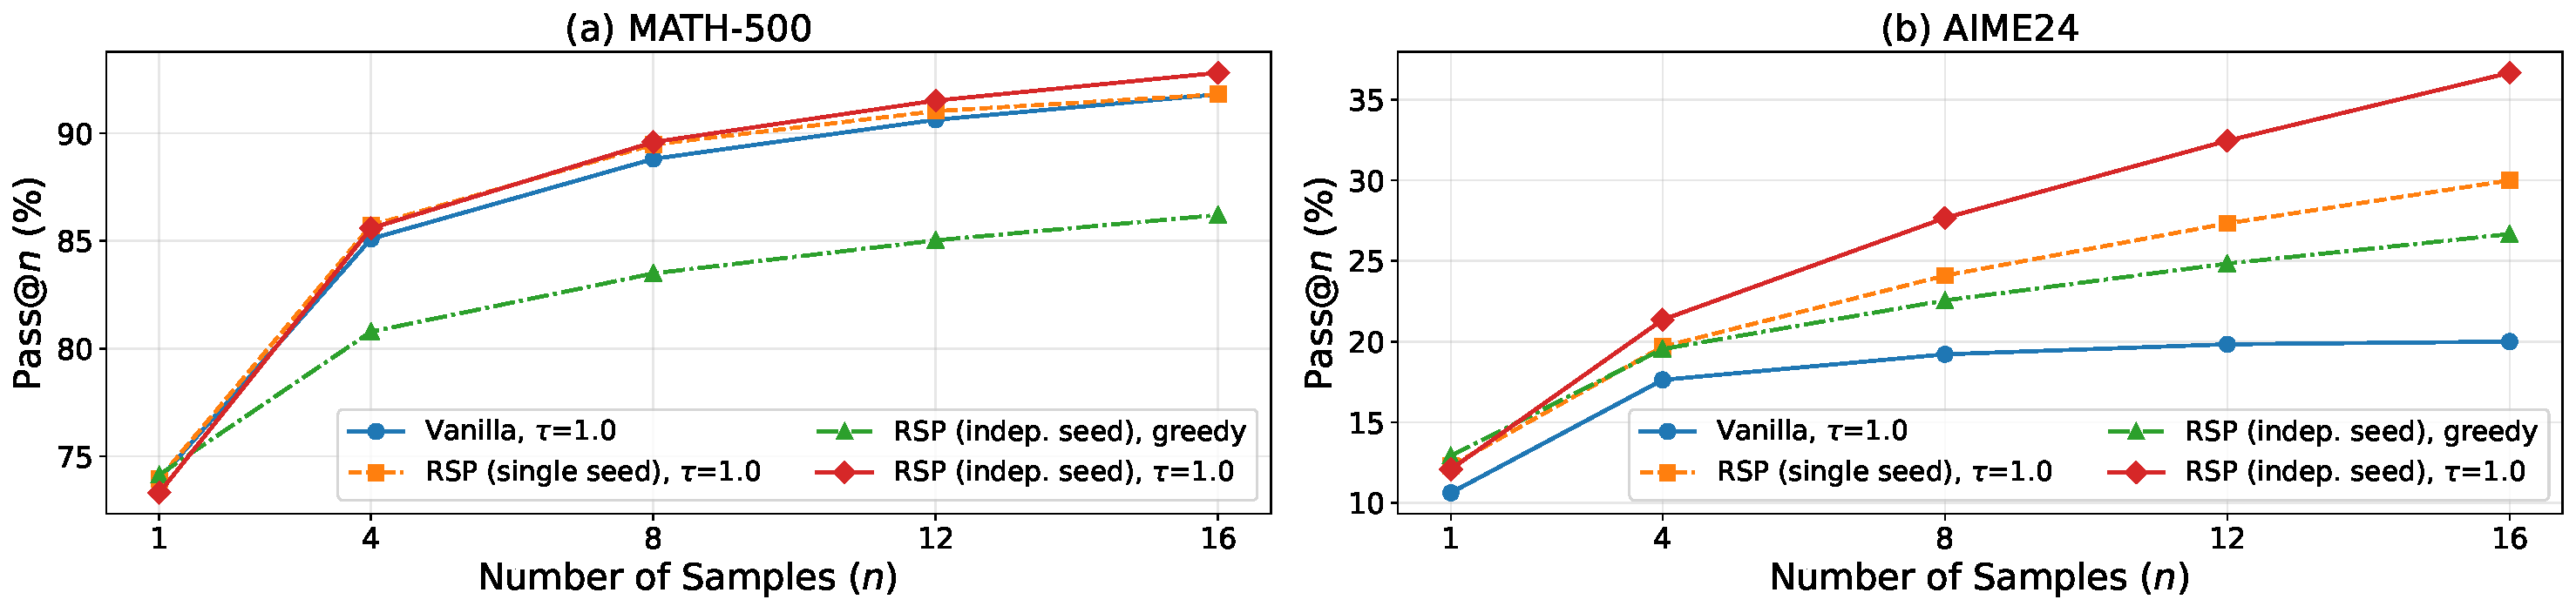
\includegraphics[width=\textwidth]{img/diversity/pass_at_n_combined.pdf}
  \caption{Pass@$n$ scaling on MATH-500 (left) and AIME24 (right) with Qwen2.5-Math-1.5B-Instruct, $n=16$ samples per problem. Baseline: temperature sampling only. Fixed seed: single RSP shared across samples combined with temperature. Indep.\ seed: a different RSP per sample, with or without temperature.}
  \label{fig:pass_at_n}
\end{figure}

Condition \textit{(iv)} achieves the highest Pass@$n$ on both benchmarks, reaching 92.80\% on MATH-500 and 36.67\% on AIME24 at $n=16$. Condition \textit{(ii)} shows no improvement over the baseline, confirming that the diversity gain originates from varying the random embeddings across samples, not from a single fixed perturbation. Pass@1 remains comparable to the baseline on MATH-500, and on the more challenging AIME24, \textit{(iv)} achieves higher Pass@1 than the baseline. Independent RSPs combined with temperature sampling produce the most diverse reasoning trajectories while maintaining or improving single-sample accuracy.

\paragraph{Synthesis across the three levels.}
The three analyses converge on a consistent picture. At the token level, RSP induces support expansion concentrated at the first token and decaying monotonically across steps. At the trajectory level, this localized perturbation translates into distinct reasoning strategies (large inter-cluster separation) while preserving local coherence within each strategy (unchanged intra-cluster distance). At the outcome level, the resulting trajectories cover more correct solutions without sacrificing single-sample accuracy.
